\subsection{Definitions}
\begin{enumerate}
	\item $f(x_0, y_0)$ is a local maximum of $f$ if for some $\delta > 0$, $f(x_0, y_0) \geq f(x, y) \forall (x,y) \in N((x,y),\delta)$.
		That is, you can draw a circle in the domain of $f$ centered at $(x_0, y_0)$ such that the value of $f$ at every point in the circle besides $(x_0, y_0)$ is less than $(x_0, y_0)$.
	\item $f(x_0, y_0)$ is a local minimum of $f$ if for some $\delta > 0$, $f(x_0, y_0) \leq f(x,y) \forall (x,y) \in N((x,y),\delta)$.
		That is, you can draw a circle in the domain of $f$ centered at $(x_0, y_0)$ such that the value of $f$ at every point in the circle besides $(x_0, y_0)$ is greater than $(x_0, y_0)$.
	\item $f(x_0, y_0)$ is a global max of $f$ if $f(x_0, y_0) \geq f(x,y) \forall (x,y) \in D(f)$ where $D(f)$ is the domain of $f$.
	\item $f(x_0, y_0)$ is a global min of $f$ if $f(x_0, y_0) \leq f(x,y) \forall (x,y) \in D(f)$ where $D(f)$ is the domain of $f$.
\end{enumerate}
\begin{theorem}
	If $(x_0, y_0)$ is in the domain of $f$ and a local extrema of $f(x,y)$, then $f_x(x_0, y_0)$ and $f_y(x_0, y_0)$ is either 0 or undefined.
\end{theorem}

\begin{figure}[H]
	\centering
	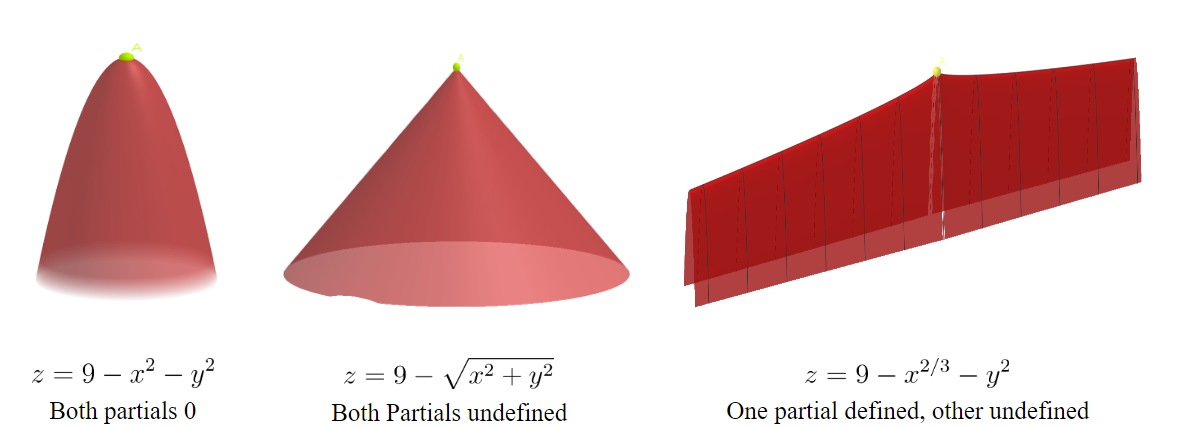
\includegraphics[width=0.9\textwidth]{./differentialMultivariableCalculus/optimization.png}
	\caption{Critical points appear when the partial derivatives are 0 or undefined.}
\end{figure}